%% Copyright 2019 Matheus H. J. Saldanha <mhjsaldanha@gmail.com>
%
% This work may be distributed and/or modified under the
% conditions of the LaTeX Project Public License, either version 1.3
% of this license or (at your option) any later version.
% The latest version of this license is in
%   http://www.latex-project.org/lppl.txt
% and version 1.3 or later is part of all distributions of LaTeX
% version 2005/12/01 or later.
%
% This work has the LPPL maintenance status `maintained'.

\documentclass[12pt,a4paper]{article}
% Pacotes para o português.
\usepackage[english]{babel}
\usepackage{listings}
\usepackage[utf8]{inputenc}
\usepackage[T1]{fontenc}
\usepackage{graphicx}     % Comando \includegraphics
\usepackage{float}
\usepackage{xcolor}       % Comando de cores \textcolor
%\usepackage{indentfirst}  % Indenta o primeiro parágrafo de cada seção
\usepackage{url}          % Comandos \url e \href
\usepackage[top=2cm, bottom=2cm, left=2cm, right=2cm]{geometry} % Define as margens do documento
\usepackage{multirow}     % Permite criar tabelas com uma célula ocupando várias linhas
\usepackage{amssymb}      % Símbolos matemáticos
\usepackage{amsmath}      % Ambientes para escrever fórmulas, \begin{align} por exemplo.
\usepackage{caption}      % Para definir o estilo das legendas de figuras e tabelas.
%\usepackage{setspace}     % Para definir espaçamento entre linhas. (\onehalfspacing, \singlespacing, \doublespacing)
\usepackage{breakcites}   % Para permitir quebra de linha no meio de citações.
\usepackage{times}        % Fonte Times New Roman
\usepackage{lipsum}       % Para gerar texto temporário. Exemplo: \lipsum \lipsum[1] \lipsum[4-5].
\usepackage{inconsolata}  % Fonte boa para códigos e URLs. Use \texttt{}
\usepackage{hyperref}     % Faz os links ficarem azuis e clicáveis. Facilita a navegação pelo PDF.
\usepackage{enumerate}

\makeatletter
\hypersetup{
	pdfkeywords={research project},
	colorlinks=true,       		% false: boxed links; true: colored links
	linkcolor=blue,          	% color of internal links
	citecolor=blue,        		% color of links to bibliography
	filecolor=magenta,      	% color of file links
	urlcolor=blue,
	bookmarksdepth=4,
}
\makeatother

\makeatletter
\renewcommand\tableofcontents{%         % Redefine table of contents to our taste
    \section*{\huge\centering\contentsname
        \@mkboth{%
           \MakeUppercase\contentsname}{\MakeUppercase\contentsname}}%
           \vspace{24pt}%
    \@starttoc{toc}%
    \newpage%
}

% Comando para marcar o texto para revisão.
\newcommand{\rev}[1]{\textcolor{red}{#1}}

% Permite escrever aspas normais "text" em vez de ``text''
\usepackage[autostyle]{csquotes}
\MakeOuterQuote{"}

\pagenumbering{roman}
\begin{document}

\doublespacing

\begin{titlepage}
    \begin{center}
        {\large \sc INDIAN INSTITUTE OF TECHNOLOGY BOMBAY} \\
        \begin{figure}[H]
            \centering
            
\includegraphics[width=0.5\textwidth]{text/IITB_logo.png}\\
            %\caption{}
            %\label{fig:my_label}
        \end{figure}        
        
        {\small \sc DEPARTMENT OF AEROSPACE ENGINEERING}
        
        \vspace{1.5cm}
        \rule{\linewidth}{1pt}
        
        \vspace{0.7em} % Ajuste ao seu gosto
        {\Large \fseries SIMULATION OF COMPRESSIBLE FLOWS USING SU2}
        \vspace{0.2em} % Ajuste ao seu gosto
        
        \rule{\linewidth}{1pt} \\
        {\small \sc SUPERVISED LEARNING PROJECT}
    \end{center}
    
    \vspace{2.8cm}

       \begin{minipage}{0.43\textwidth}
        \emph{Submitted by:}\\
        %\rule{0.9\linewidth}{0.3mm}\\
        M Vishnu Sankar
    \end{minipage}
    \hspace{4cm}
    \begin{minipage}{0.43\textwidth}
        \emph{Supervisor:}\\
        %\rule{0.9\linewidth}{0.3mm}\\
        Prof. Kowsik Bodi
    \end{minipage}

    \vfill

    % Data
    \begin{center}
        \makeatletter
         December 2020
        \makeatother
    \end{center}
\end{titlepage}

\noindent{}
\pagestyle{empty} 
\tableofcontents
\newpage
\setcounter{page}{1}
\pagestyle{plain}
\listoffigures
\cleardoublepage

\listoftables
\cleardoublepage

\pagenumbering{arabic}
%\pagestyle{empty}
\begin{center}
    {\bf \huge Abstract} \\[2em] 
\end{center}
The prime objective of this Supervised Learning Project is to get an overview of high speed flow simulations using the CFD software SU2. Firstly it delves into the features used in SU2 through a simple inviscid simulation, various numerical methods used in SU2 and finally we look at the simulation of flow through optimum expanded, under-expanded and over-expanded nozzle. Then the Method of Characteristics is used to design a minimum length nozzle.

\section{Introduction}
\label{section:Introduction}
\subsection{Fundamentals of SU2}
SU2 is an open source software built using C++ and Python for largely solving problems pertaining to Computational Fluid Dynamics and also other domains such as electrodynamics, elasticity etc. SU2 makes use of the Finite Volume Solver for most of the fluid flow problems. In this report the flow is assumed to be Euler to reduce complexity. 
\subsubsection{Markers \& Boundary Conditions}
Farfield: If a marker is assigned as Farfield no specific value is imposed on the marker and the governing equations are solved to arrive at the values of the flow variables. Generally inlet is defined as farfield  for external flow problems and the free-stream values are assigned for the flow variables at the inlet. \textbf{Free-stream} values are also used as \textbf{initial conditions}, so it is necessary to define free-stream values \\
\\
Total Conditions: Total Conditions is primarily used at the inlet to define the total temperature, total pressure, unity velocity vector to define the flow direction. A typical example of Total Condition\\
MARKER\_INLET = ($Inlet_1$, $T_0$ , $P_0$, $\hat {v_x}$, $\hat{v_y}$, $\hat{v_z}$) \\
\\
Pressure Outlet: Defines the exit static pressure at the outlet\\
MARKER\_OUTLET = (Outlet, P)\\
\\
The biggest disadvantage is that SU2 doesn't provide a velocity inlet option for compressible flows\\

\subsubsection{Convergence Criteria}
Steady-State Residual: If the convergence criteria is a residual, the solver stops once the computed residual is smaller than the value set by the user.\\
\\
Steady-State Coefficient: If  the  convergence  criteria  is  a coefficient,  a cauchy series approach  is  used for which a cauchy element is defined as the difference between coefficients of consecutive iterations.  When the average over a certain number of elements is below the value set by the user the solver stops iterating. \\
\\
Maximum Iteration: The user can also define the maximum number of iterations, if the solver encounters this limit then it automatically quits the iteration even if the residuals are not converged.\\

\subsection{Convective Schemes}
JST: The Jameson-Schmidt-Turkel scheme is a second order accurate central scheme. \\
\\
ROE: ROE is a second order accurate unpwind scheme, for the linear advection equation the information travels in the direction of the characteristic speed. If $a \geq 0$ then the information travels from the $i^t^h$ to the $(i+1)^t^h$ coordinate in the stencil \\
\\
HLLC: HLLC is also an upwind second order scheme\\
\subsubsection{Other Features}
Multigrid:
The {\textit{multigrid algorithm}} is used for accelerated convergence, it automatically agglomerates the original mesh into a series of coarser representation and smoothing iterations are performed on all mesh levels with each non-linear solver iteration in order to provide a better residual update. A multigrid with X levels implies there are X coarser mesh levels and 1 level for the original mesh. {W\_CYCLE} provides better convergence rates though it is more computationally intensive.\\
\\
Windowing Functions for Unsteady Flows:\\
\begin{equation}
        C_D = 1/M\int_{0}^{M}w(t/M)C_D(t) dt 
    \end{equation}
    A windowing function is zero on boundaries and has an integral value of 1.  "WINDOW\_START\_ITER" must start once the transient phase of flow begins. Su2 offers several window functions with which the time-averaged value converges faster
\begin{table}[ht]
        \centering
        \scalebox{0.75}{
        \begin{tabular}{|l|c|}
        \hline
        WINDOW\_FUNCTION & CONVERGENCE ORDER\\
        \hline
        SQUARE & 1\\
        \hline
        HANN & 3 \\
        \hline
        HANN\_SQUARE & 5 \\
        \hline
        BUMP & Exponential \\
        \hline
        \end{tabular}}
        \caption{Windowing Functions}
        \label{tab:Windowing Functions}
\end{table}\\
CFL Adaptive:
The CFL adaptive feature can be turned ON or OFF. It controls the multiplicative factors to increase or decrease the CFL with each iteration (depending on the success of each nonlinear iteration). $CFL_i$ is given by $CFL_i_-_1(Residual_i_-_1/Residual_i)^n$
%\footnote{Veja, por exemplo, \url{http://www.fapesp.br/10408}.}
\newpage

\section{Comparing Various Numerical Schemes}
\label{section:Comparing the Numerical Scheme}
\subsection{Grid Independence Test}
Firstly a Grid Independent Test was carried out to find the approximate number of cells to run an economical simulation and finally the mesh with 15000 number of cells was chosen.
\begin{table}[ht]
    \centering
    \scalebox{1.00}{
    \begin{tabular}{|c|c|}
     \hline
     M_\infty & 2.0  \\
     \hline
     P_\infty & 10^5  \\
     \hline
     T_\infty & 300  \\
     \hline
    \end{tabular}}
    \caption{Free-stream Value}
    \label{tab:Free-stream Value}
    \vspace{8mm}
     
    \centering
    \scalebox{1.00}{
    \begin{tabular}{|c|c|}
     \hline
     M_2 &  1.64052 \\
     \hline
     P_2 & 170658 Pa \\
     \hline
     T_2 & 351.045 K  \\
     \hline
     Shock angle &  39.3134  \\
     \hline
    \end{tabular}}
    \caption{Theoretical Values from Oblique Shock relation}
    \label{tab:Theoretical Values}
    \vspace{8mm}
    
    \centering
    \scalebox{1.00}{
    \begin{tabular}{|l|l|}
     \hline
     Solver & Euler  \\
     \hline
     Num\_Method\_Grad & Weighted\_Least\_Squares  \\
     \hline
    Conv\_Num\_Method\_Flow & \textbf{HLLC}  \\
     \hline
    CFL & 5\\
     \hline
     Time\_Diecre\_Flow & Euler\_Implicit\\
     \hline
    Conv\_Field & RMS\_Density\\
     \hline 
    Conv\_Residual\_Minval & -13 (log_1_0)\\
     \hline 
    Conv\_Cauchy\_Eps & 1E-10 (last 100 elements)\\
     \hline
    \end{tabular}}
    \caption{Setup}
    \label{tab:Setup}
    \vspace{8mm}

    \centering
    \begin{tabular}{|l|l|l|l|l|}
    \hline
    Mesh Cells & M_2 & P_2 & T_2 \\
    \hline
    90000 & 1.6431X & 17073X & 351.09X \\
    \hline
    30000 & 1.6431X & 17073X & 351.09X \\
    \hline
    15000 & 1.6431X & 17073X & 351.09X \\
    \hline
    7500 & 1.643XX & 1707XX & 351.0XX \\
    \hline
    1900 & 1.64XXX & 1707XX & 351.0XX\\
    \hline
    \end{tabular}
    \caption{Comparison}
    \label{tab:Comparison}
\end{table}\\
\newpage
\\
\begin{figure}[H]
\centering
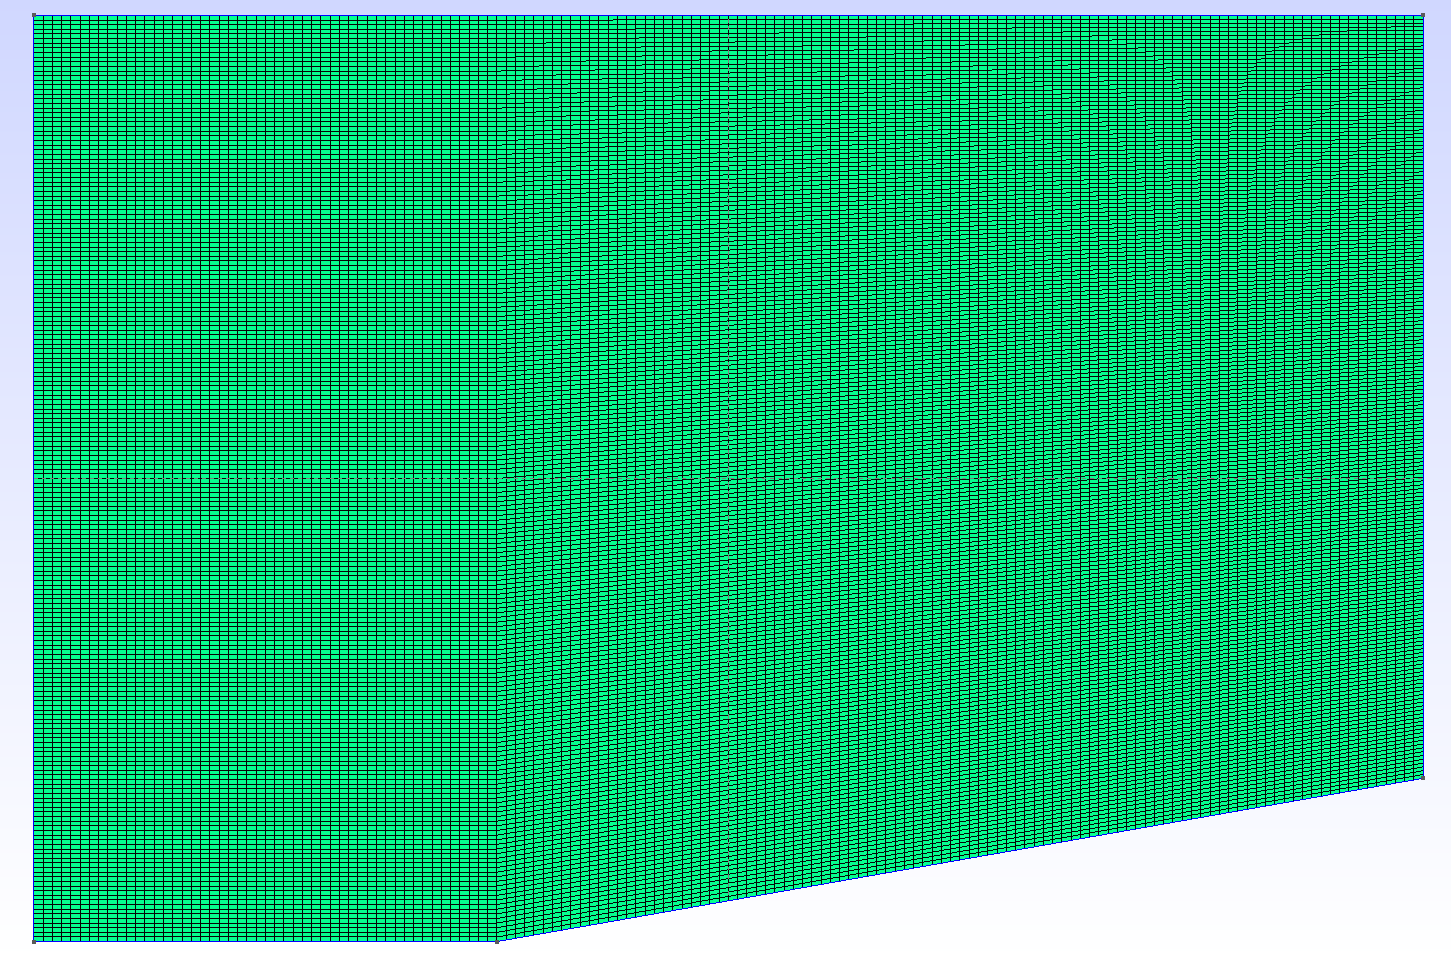
\includegraphics[width=0.8\textwidth]{text/inviscid_wedge_fine_mesh.png}\\
\caption[Inviscid Mesh]{Mesh: 30,000 Cells | Generated in Gmsh}
\label{fig1.1: Inviscid Mesh}
\end{figure}
\\
\begin{figure}[H]
\centering
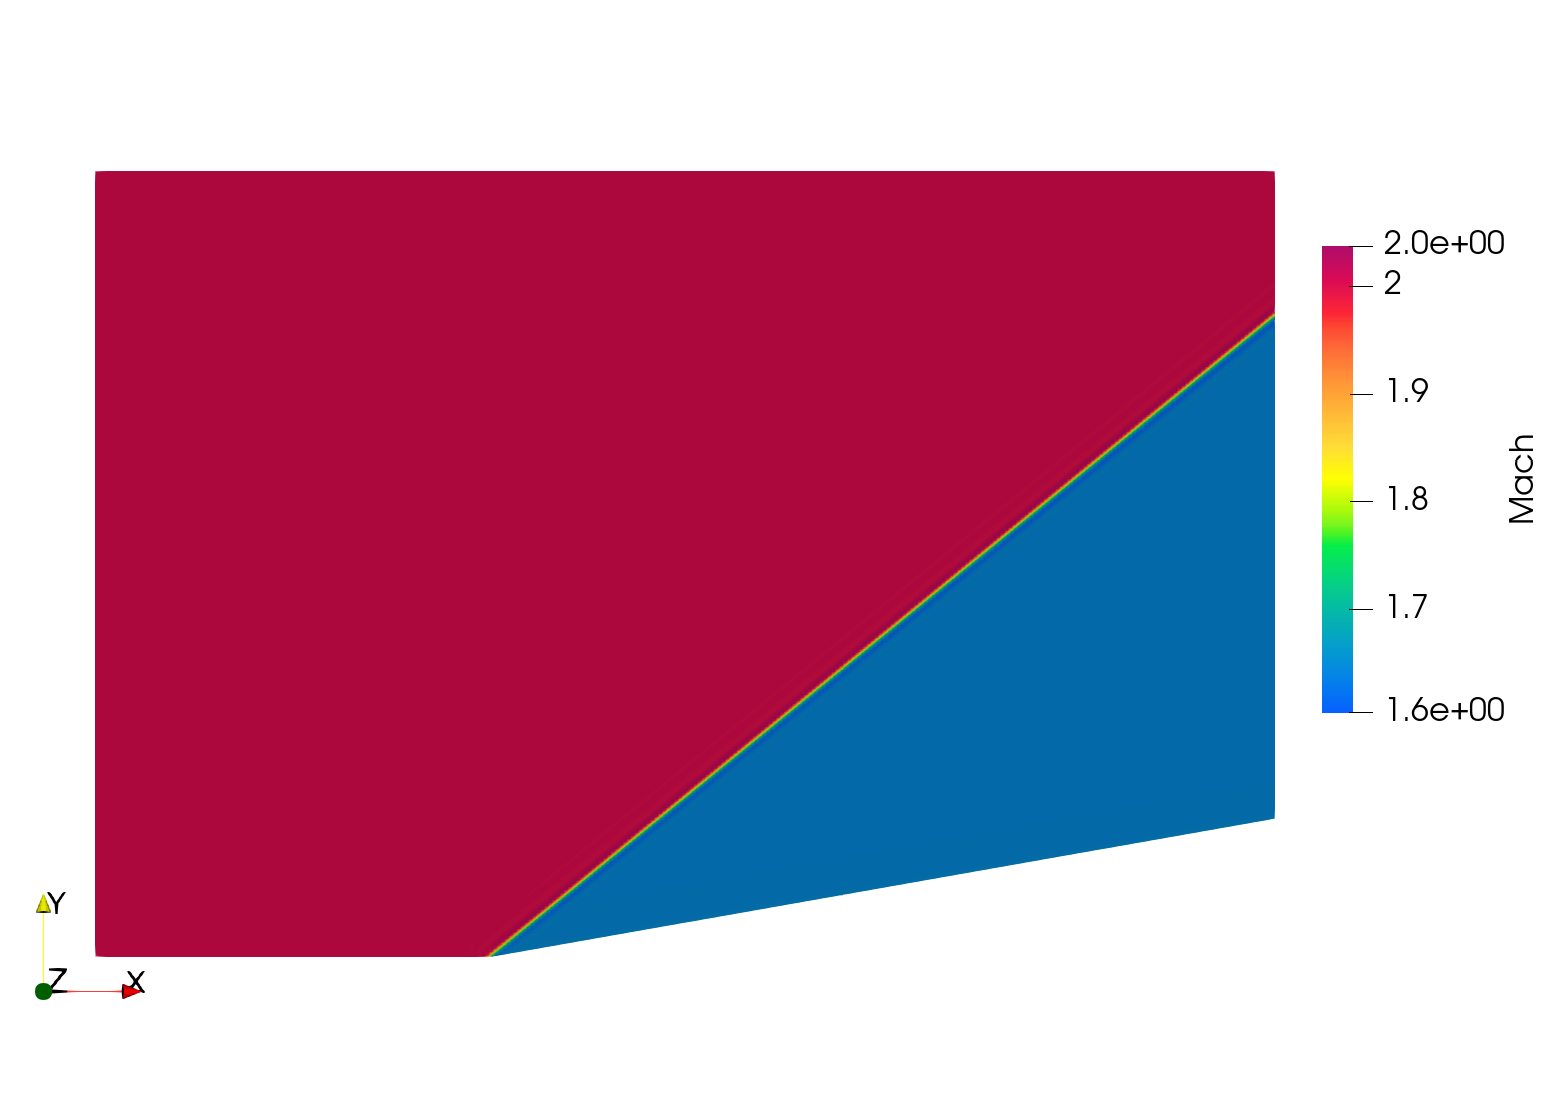
\includegraphics[width=0.8\textwidth]{text/Mach_HLLC_Inviscid_Wedge.png}\\
\caption[Inviscid Mach Contour]{Mach Contour}
\label{fig: Inviscid Mach Contour}
\end{figure}

\begin{figure}[H]
\centering
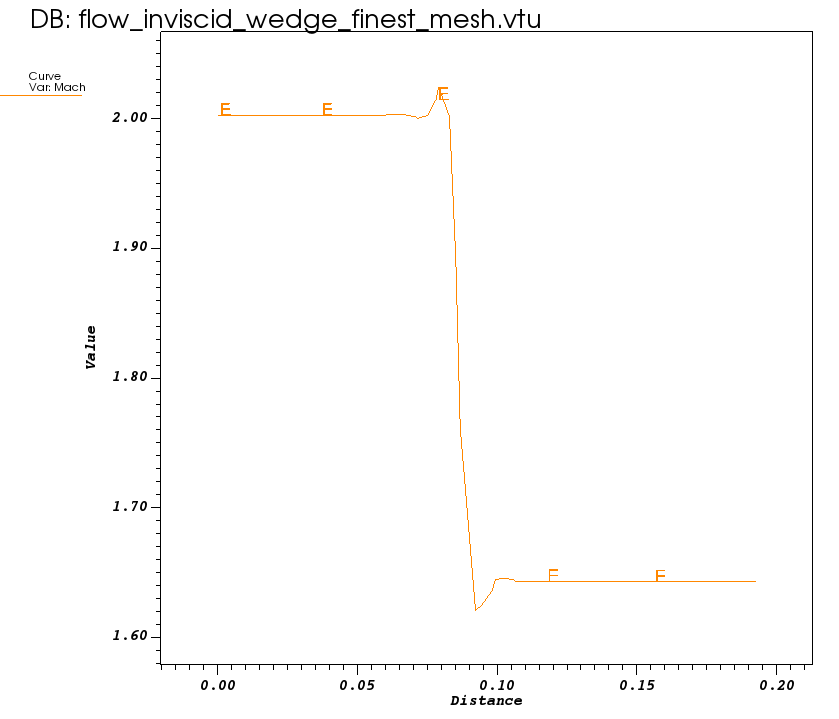
\includegraphics[width=0.6\textwidth]{text/Mach_Per_Shock_Inviscid_Wedge.png}\\
\caption[HLLC - Mach vs. X]{HLLC - Mach vs. X}
\label{fig: Mach vs. X}
\end{figure}

\begin{figure}[H]
\centering
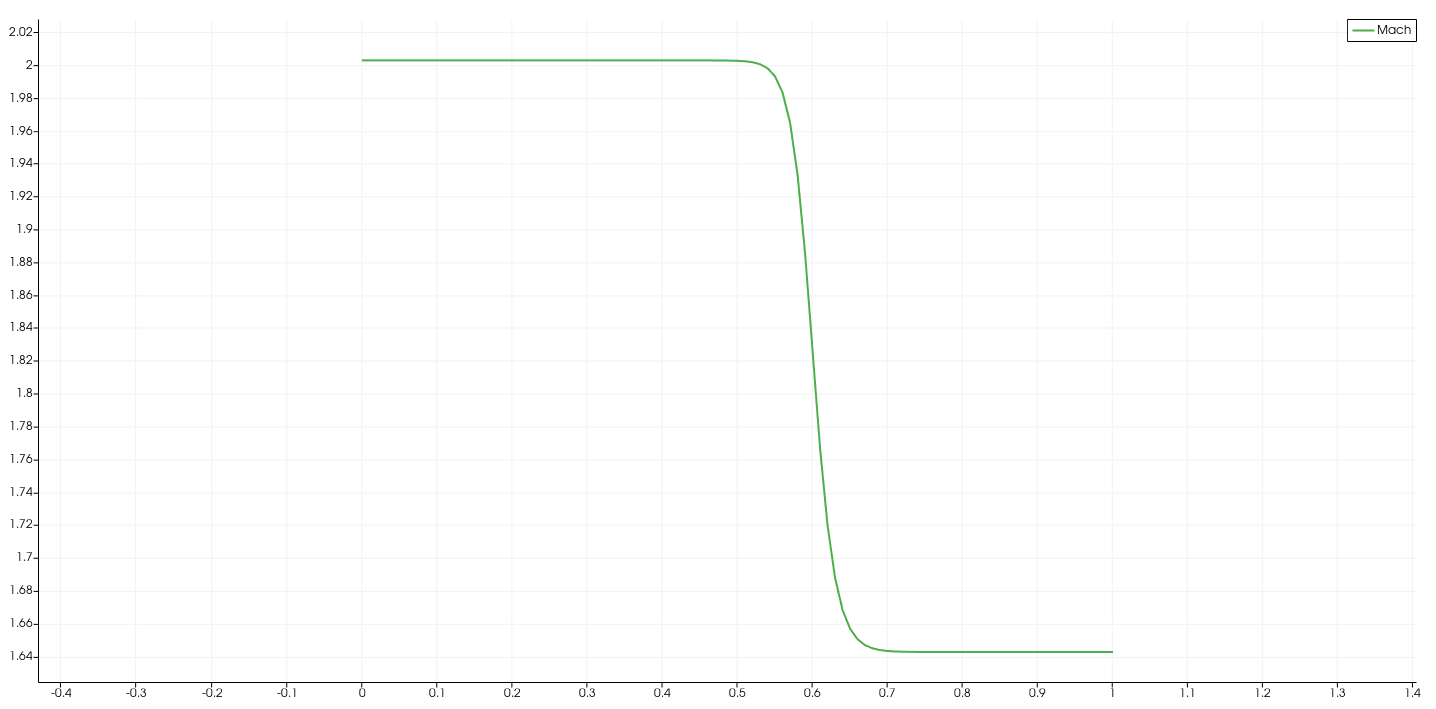
\includegraphics[width=0.8\textwidth]{text/Lax_M_vs_X_Inviscid_Wedge.png}\\
\caption[Lax-Friedrich - Mach vs. X]{Lax-Friedrich - Mach vs. X}
\label{fig: Lax-Friedrich - Mach vs. X}
\end{figure}
\\
Post-Processing: The theoretical value of shock angle is $39.314^0$, but the value from the simulation is $40.019^0$. This was found using the density gradient, where the maximum value of the gradient was calculated at the shock, since the maximum gradient has to be perpendicular to the shock, $90^0$ was added to the gradient angle to find the shock angle. The shock angle was averaged over four such values calculated from five different horizontal lines passing through the shock with a spacing of 0.005 units along the y-axis. The error in shock angle is 1.80\%. \\
\begin{center}
$ \triangledown \rho = \frac{d\rho}{dx} \hat{i} + \frac{d\rho}{dy} \hat{j}  $\\
$ |\triangledown \rho| = \sqrt{(\frac{d\rho}{dx})^2  + (\frac{d\rho}{dy})^2 } $ \\
$ \theta_{shock} = \frac{\pi}{2} + \arctan{(\frac{d\rho/dy}{d\rho/dx})}$ at $|\triangledown \rho|_{max} $
\end{center}
\newpage
The data from the numerical schemes were extracted and plotted for comparison
\begin{figure}[H]
    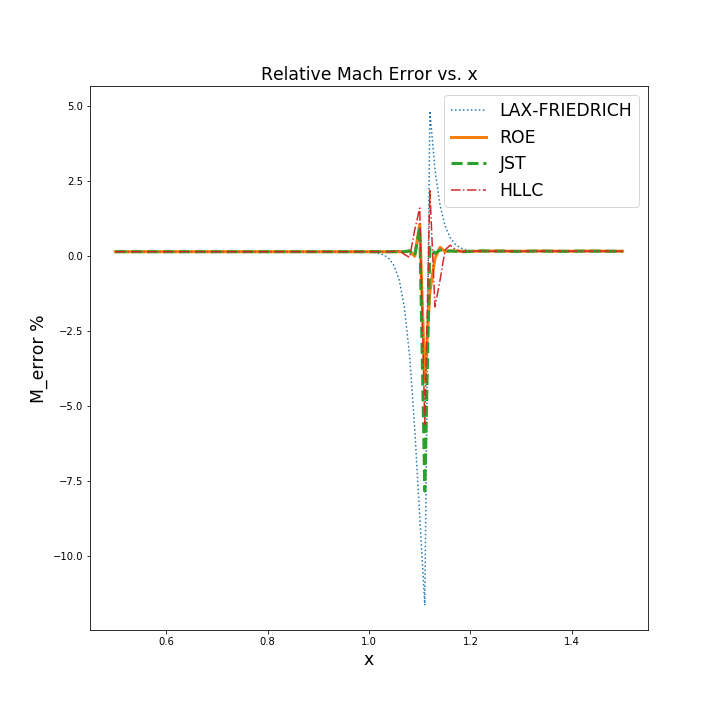
\includegraphics[width=0.5\textwidth]{text/M_error_comparison.png}
    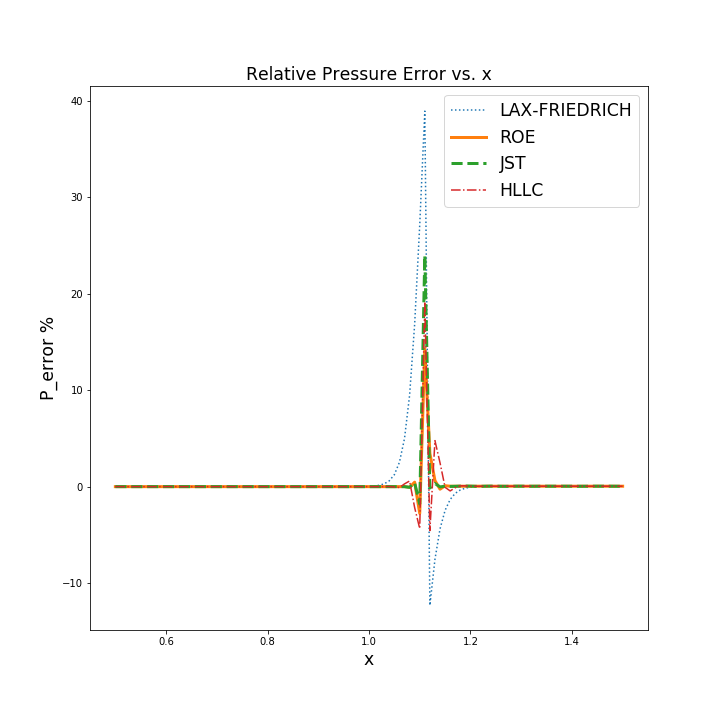
\includegraphics[width=0.5\textwidth]{text/P_error_comparison.png}
    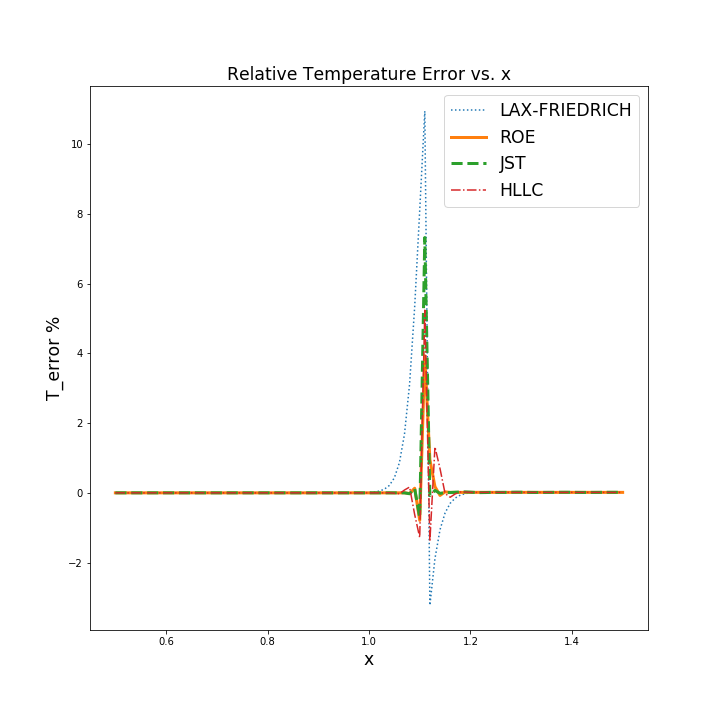
\includegraphics[width=0.5\textwidth]{text/T_error_comparison.png}
    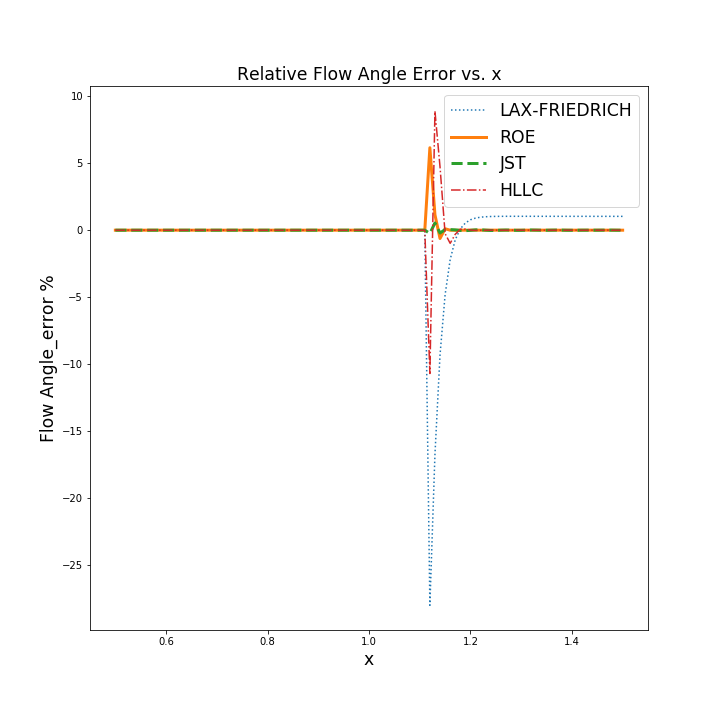
\includegraphics[width=0.5\textwidth]{text/FA_error_comparison.png}
    \caption[Errors associated with the Numerical Scheme]{Errors associated with the Numerical Scheme}
    \label{fig:Errors associated with the Numerical Scheme}
\end{figure}
From the plots shown above the ROE scheme seems to have the least error, followed by the HLLC scheme, but it is computationally expensive, so the HLLC scheme was chosen for its faster convergence and accurate results\\
\begin{table}[h]
    \centering
    \begin{tabular}{|l|l|l|l|l|l|}
    \hline
    Convective NM & M_2 & P_2 & T_2 & Time(sec)\\
    \hline
    JST & 1.643XX & 1707XX & 351.0XX & 644.16\\
    \hline
    LAX\_FRIEDRICH & 1.642XX & 17075X & 351.XXX & 197.6\\
    \hline
    HLLC & 1.6431X & 17073X & 351.09X & 106.75\\
    \hline
    ROE & 1.6431X & 17073X & 351.09X & 553.2\\
    \hline
\end{tabular}
    \caption{Comparison between Convective NM}
    \label{tab:Comparisonbetween Convective NM }
\end{table}
\newpage
\begin{figure}
    \centering
    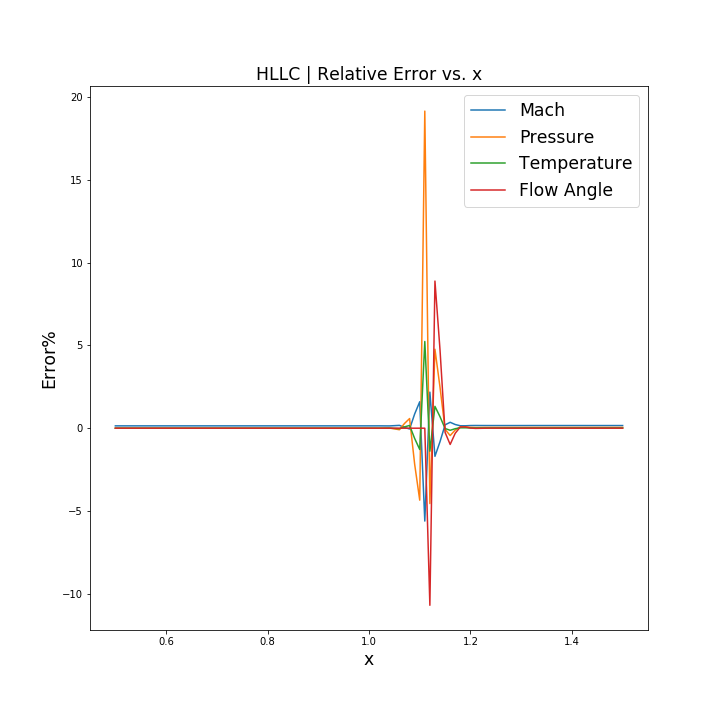
\includegraphics[width=0.75\textwidth]{text/error_HLLC.png}   
    \caption[HLLC - Relative Error]{Relative Error in flow variables}
    \label{fig:HLLC - Relative Error}
\end{figure}

\subsection{Time vs. CFL}
In this section, for a constant number of cells, the optimum CFL number is found by plotting Time vs. CFL number, which has the minimum computational cost. And then the number of mesh cells is quadrupled to test if the same trend continues.\\
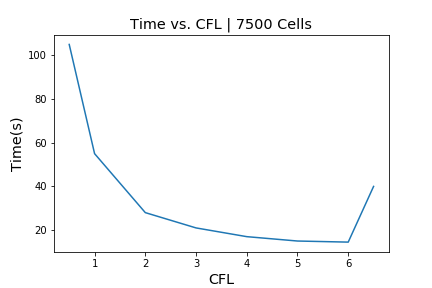
\includegraphics[width=0.5\textwidth]{text/time_vs_CFL_7500_Cells.png}
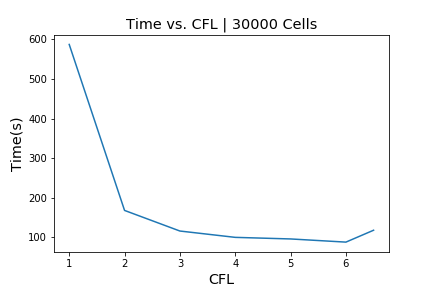
\includegraphics[width=0.5\textwidth]{text/time_vs_CFL_30000_Cells.png}\\
For CFL values lesser than 1, the convergence is so slow that even after 10000 iterations the residual were far from the convergence criteria. For CFL values greater than 7, the residual initially oscillates around and then later diverges.\\
\newpage

\section{Nozzle Simulations}
\label{section:hpc}
\subsection{Optimum Nozzle Expansion}
Quasi 1-D Theory: The quasi 1-D theory is used for verification purposes, which assumes that all the variables are only a function of x, the below equation can be derived from invoking mass conservation and isentropic conditions\\
\begin{center}
    $(\frac{A}{A^*}) = \frac{1}{M^2}[1+\frac{\gamma-1}{2}M^2]^{\frac{\gamma+1}{\gamma-1}}$
\end{center}
\begin{figure}[H]
    \centering
    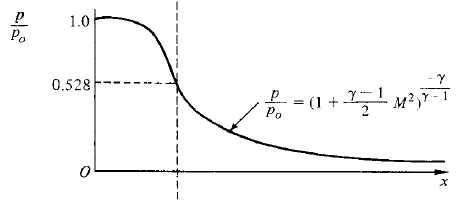
\includegraphics[width=0.5\textwidth]{text/Nozzles_Optimum.PNG}
    \caption[Variation of Pressure ratio a long center-line]{Pressure ratio vs. Center-line (Source [1])}
    \label{fig:Variation of Pressure ratio a long center-line}
\end{figure}

\begin{table}[ht]
    \centering
    \begin{tabular}{|c|c|}
    \hline
    T_{o}  &  3600 \\
    \hline
    P_{o} & 7 Mpa\\
    \hline
    P$_{e}$/P$_{th}$ & 0.0473  \\
    \hline
    A$_e$/A$_{th}$ & 3\\
    \hline
    M_{th} & 1 \\
    \hline
    M_{e} & 2.63741\\
    \hline
    P$_{e}$ & 331090.842 \\
    \hline
    T$_{e}$ & 1505.525 \\
    \hline
    \end{tabular}
    \caption{Parameters}
    \label{tab:my_label}
\end{table}

\begin{figure}[H]
    \centering
    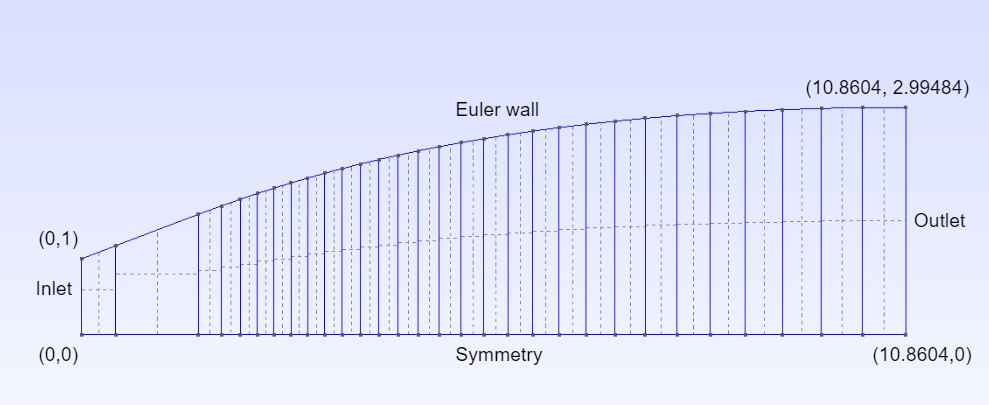
\includegraphics[width=0.75\textwidth]{text/Nozzle_Geometry.PNG}\\
    \caption[Geometry]{Geometry}
    \label{fig:Geometry}
\end{figure}
\begin{figure}[H]
    \centering
    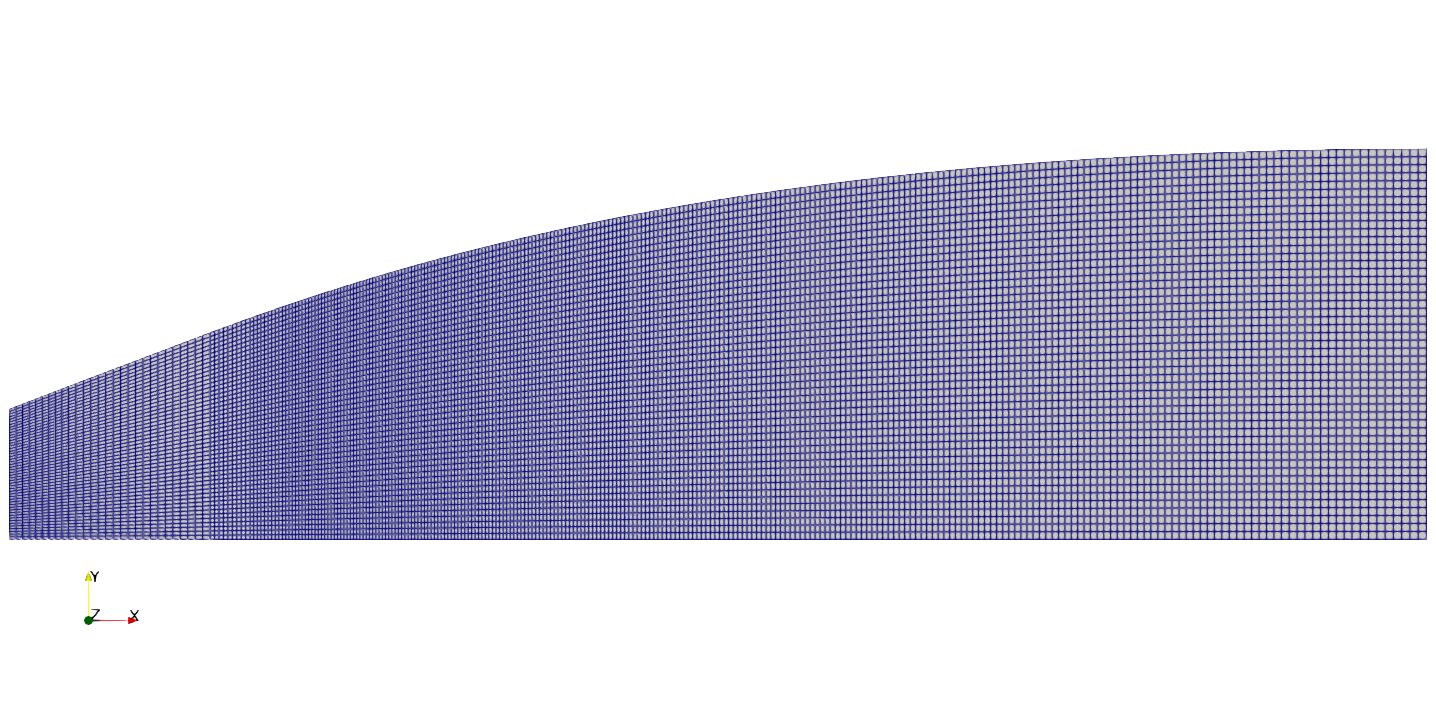
\includegraphics[width=0.8\textwidth]{text/Nozzle_mesh_pic.png}
    \caption[Mesh]{Mesh}
    \label{fig:Mesh}
\end{figure}

\begin{flushleft}
\textbf{Set-Up}\\
\end{flushleft}
\begin{center}
\begin{tabular}{|l|l|}
     \hline
     Solver & Euler  \\
     \hline
     Num\_Method\_Grad & Weighted\_Least\_Squares  \\
     \hline
    Conv\_Num\_Method\_Flow & \textbf{JST}  \\
     \hline
    CFL & 5\\
     \hline
     Time\_Diecre\_Flow & Euler\_Implicit\\
     \hline
    Conv\_Field & RMS\_Density\\
     \hline 
    Conv\_Residual\_Minval & -12 (log_1_0)\\
     \hline 
    Conv\_Cauchy\_Eps & 1E-10 (last 100 elements)\\
     \hline
\end{tabular}\\
\end{center}
\\
\\
\textbf{Initial Condition}\\
Mach$_{free-stream}$ = 1 also serves as the initial condition. In this case, this is valid as the mach number inside the nozzle is always greater than 1.\\
\\
\textbf{Solver \& Convective Numerical Scheme}\\
Euler solver is used with JST convective numerical scheme. Other than JST and Lax-Friedrich scheme only ROE scheme showed convergence with high multigrid option. Other schemes either diverged or didn't converge. The cauchy convergence criteria is used, the average of the last 100 log$_1_0$(density residual) is set less than -12 for convergence. \\
%\end{flushleft}
%The chamber temperature and pressure is 3600 k and 7 MPa. The ratio of A$_e$/A$_t$ is 3:1. The inlet is the throat with speed of flow as M = 1. The outlet pressure is 331090.842 Pa, temperature is 1505.525 and mach number is 2.63741 as calculated using the quasi 1-D theory. Air is chosen and the gas is assumed to be ideal, hence, specific heat ratio is 1.4 and gaseous constant is 287.
\\
\textbf{Grid Independent Test}\\
\begin{table}[ht]
    \centering
    \begin{tabular}{|c|c|c|c|c|c|c|c|}
    \hline
    No of Elements & M$_e$ & P$_e$ & T$_e$ & M$_{error}$ & P$_{error}$ & T$_{error}$ & Time\\
    \hline
       73755(S)  & 2.63818 & 330742 & 1505.02 & 0.045 & 0.106 & 0.034 & 580s\\
       \hline
       13720(S)  & 2.63973 & 330060 & 1504.03 & 0.104 & 0.311 & 0.100 & 53s\\
       \hline
       7630(S)   & 2.64024 & 329909 & 1503.73 & 0.123 & 0.357 & 0.120 & 25s\\
       \hline
       26324(US)   & 2.63607 & 331749 & 1506.42 &  0.051 & 0.2 & 0.120 & 75s\\
       \hline
       7053(US)   & 2.63435 & 332671 & 1507.56 & 0.116 & 0.478 & 0.135 & 10s\\
       \hline
    \end{tabular}
    \caption{S is Structured and US is Unstructured Grid}
    \label{tab:Grid Independent Test}
\end{table}
\begin{figure}[H]
    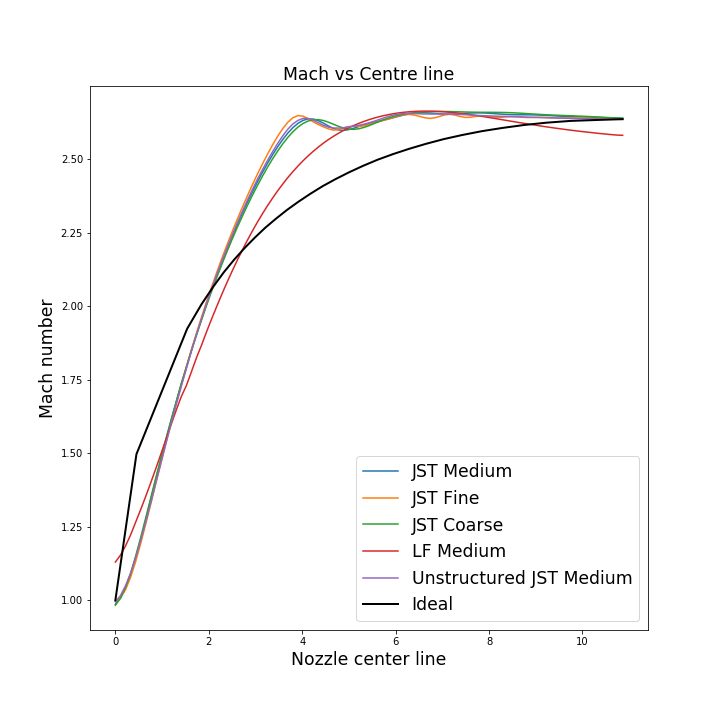
\includegraphics[width=0.5\textwidth]{text/Mach_vs_X.png}
    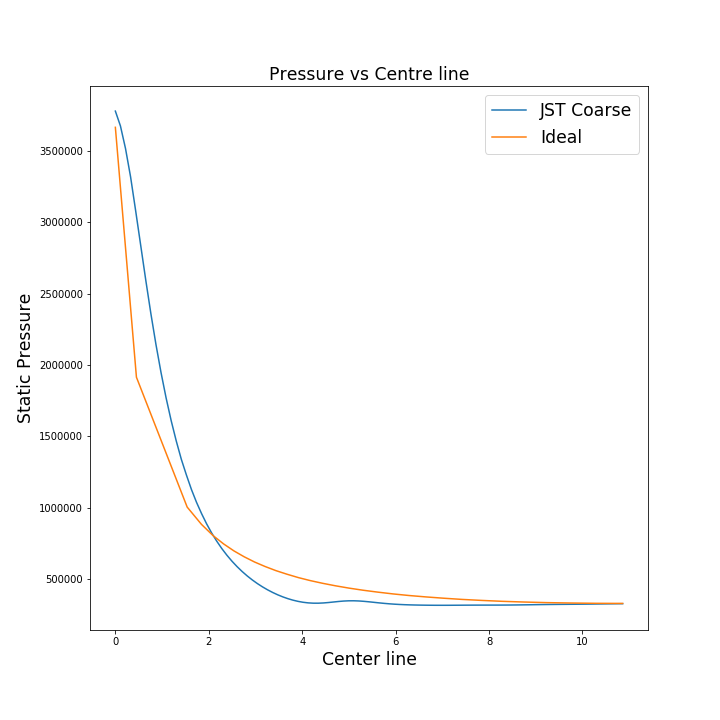
\includegraphics[width=0.5\textwidth]{text/Pressure_vs_X.png}
    \caption[Error along Center line]{Error along Center line}
    \label{fig:Error along Center line}
\end{figure}
\begin{flushleft}
\textbf{Conclusion}
\end{flushleft}
\vspace{-5}
Even though the exit parameters from the simulation are close enough to the values calculated from the quasi 1-D theory, the values in between the inlet and outlet show considerable deviation. \\
\begin{figure}[H]
    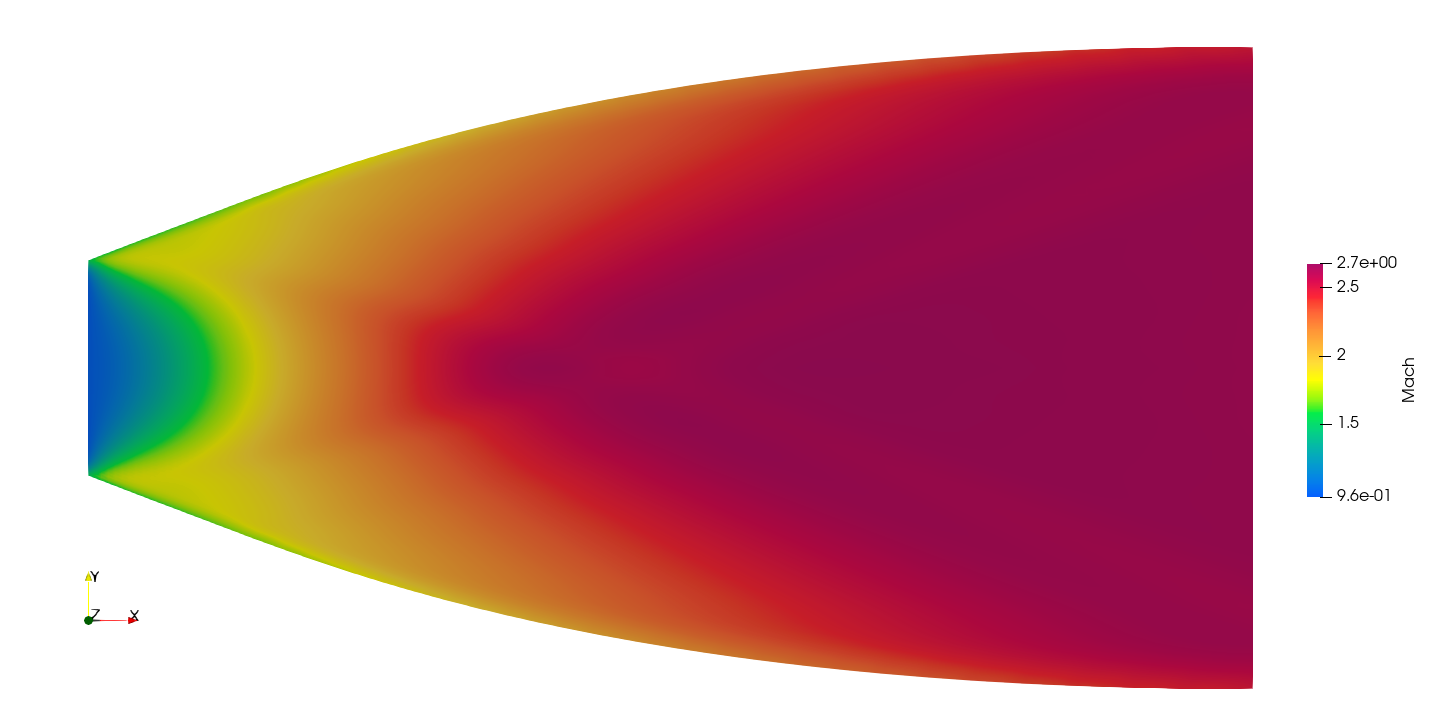
\includegraphics[width=0.5\textwidth]{text/Coarse_JST_Mach.png}
    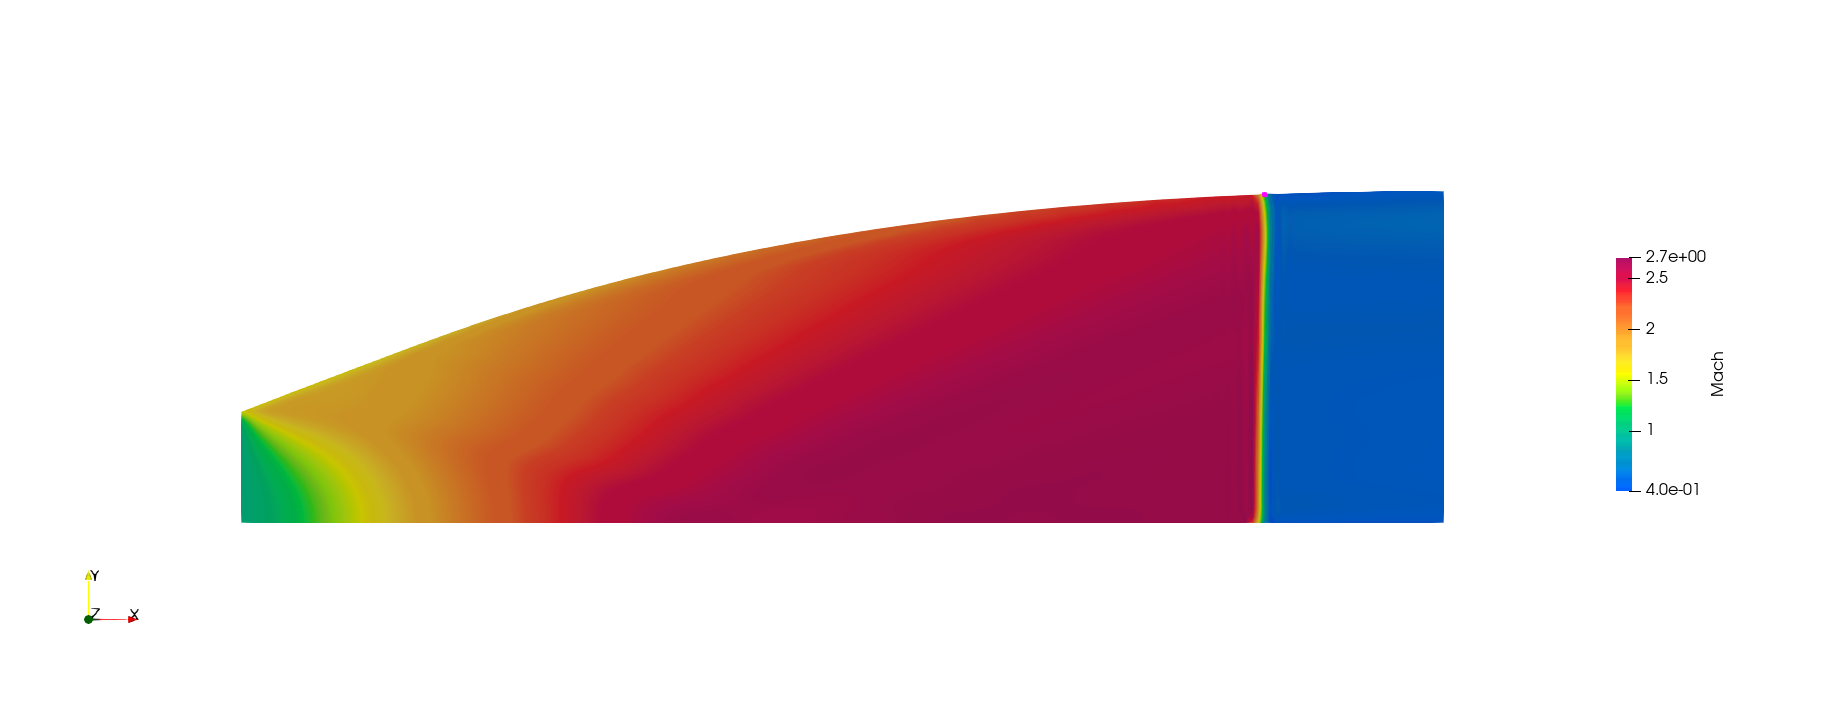
\includegraphics[width=0.5\textwidth]{text/NS_Loc.png}
    \caption[Mach Contour of flow through nozzle]{Mach Contour using JST Scheme}
    \label{fig:Mach Contour using JST Scheme}
\end{figure}

\newpage
\subsection{Extended Nozzle Simulations}
\textbf{Theory}\\
\begin{figure}[H]
    \centering
    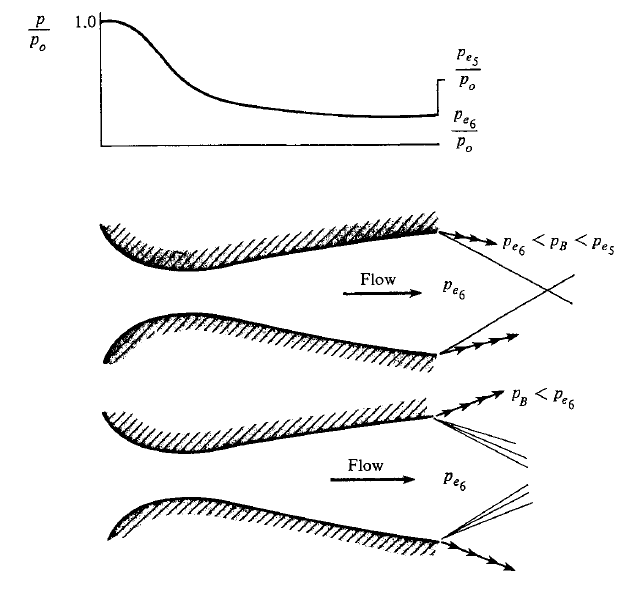
\includegraphics[width=0.6\textwidth]{text/Nozzles_Expansions.PNG}
    \caption[Over-expanded and Under-expanded Nozzle]{Over-expanded and Under-expanded Nozzle (Source [1])}
    \label{fig:Over-expanded and Under-expanded Nozzle}
\end{figure}
\textbf{Geometry}\\
\begin{figure}[H]
    \centering
    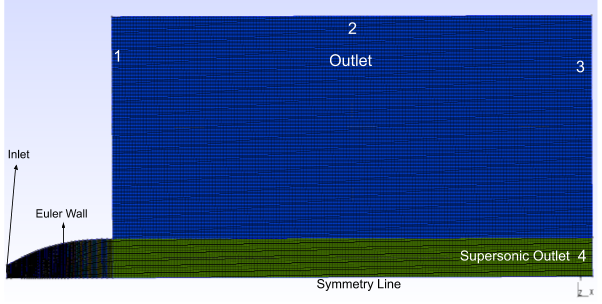
\includegraphics[width=0.75\textwidth]{text/Failed_BC.png}
    \caption[Extended Mesh of Nozzle Simulation]{Mesh}
    \label{fig:Mesh}
\end{figure}
\begin{flushleft}
\textbf{Impact of Boundary Conditions \& Initial Conditions on the Result}
\end{flushleft}
For an optimum expanded nozzle the \textbf{Outlet} is assigned a back-pressure that equals P$_{e6}$. The is a \textbf{pressure outlet} boundary condition. Since there is no velocity inlet option for compressible flows, P$_0$ and T$_0$ are assigned at the inlet. For a rocket engine that is just about to start the natural initial condition is that the speed is zero everywhere and the pressure is P$_{e6}$ and temperature is same as the atmospheric temperature. There is \textbf{NO OPTION} in SU2 to simultaneously assign Mach 1 at the inlet and Mach 0 to the rest of the domain as the initial conditions. This simulation always resulted in divergent issues or the residual oscillates continuously without a proper velocity field. To solve this issue several approaches were tried out.\\
\\
(A) Supersonic Outlet:The outlet which would have supersonic flow is given outlet supersonic. Other outlets have atmospheric pressure as the BC. The atmospheric pressure is same as the nozzle outlet pressure for optimum expansion of the nozzle. \\
\begin{figure}[H]
    \centering
    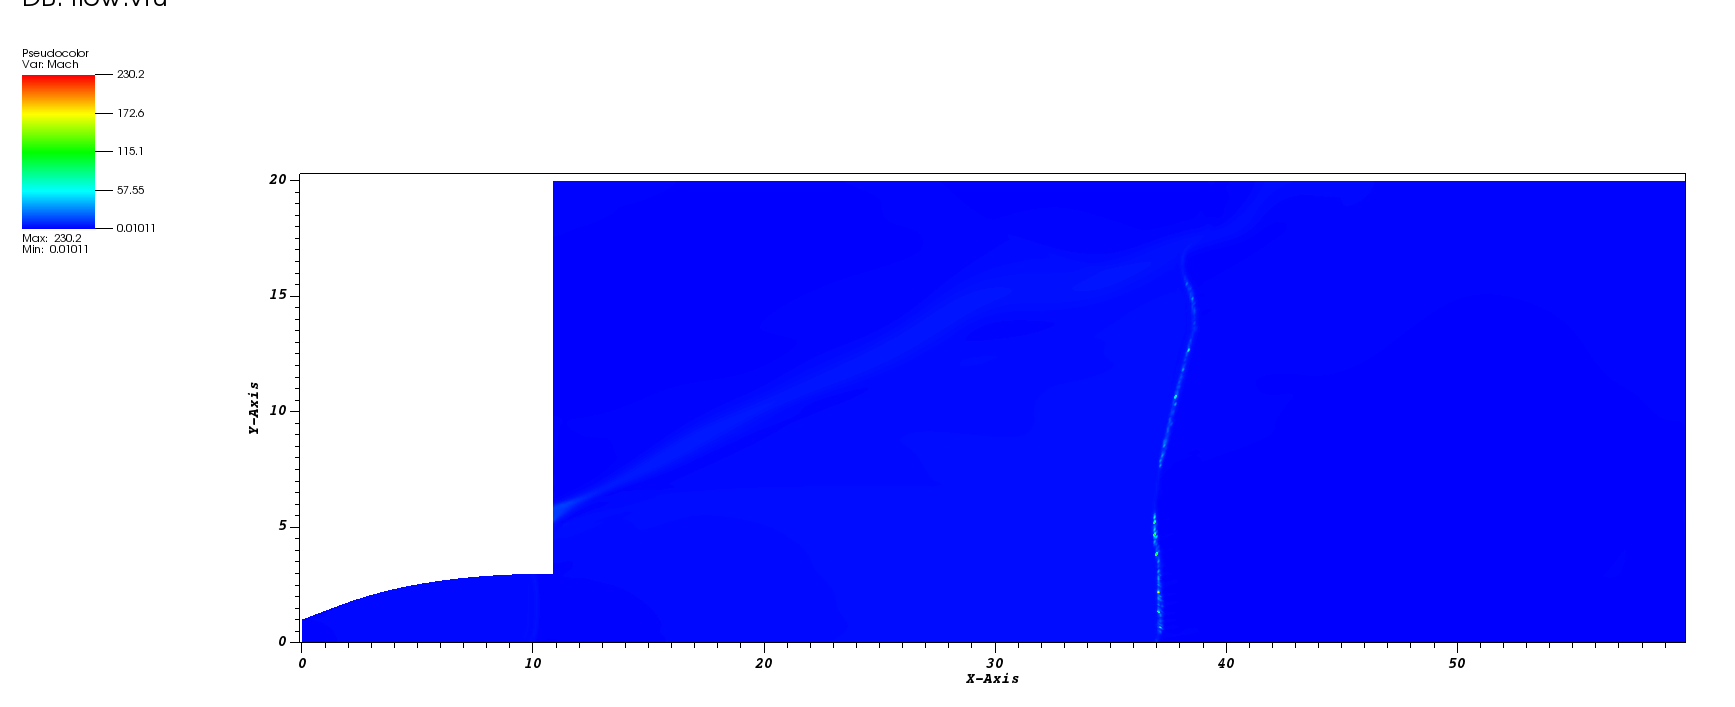
\includegraphics[width=0.55\textwidth]{text/F1.png}
    \caption[Mach Contour of Extended Mesh I]{Mach Contour}
    \label{fig:Mach Contour}
\end{figure}
The simulation resulted in residuals that oscillated continuously. diverged residuals. Different CFL values were used in the simulation, but none yielded the desired results.\\
\\
(B) Free-stream Conditions: The initial condition throughout the domain is assigned the free-stream values as shown\\
FREESTREAM\_PRESSURE = 3697972.51402 Pa\\
FREESTREAM\_TEMPERATURE = \textcolor{red}{3000 K} \\
\begin{figure}[H] 
    \centering
    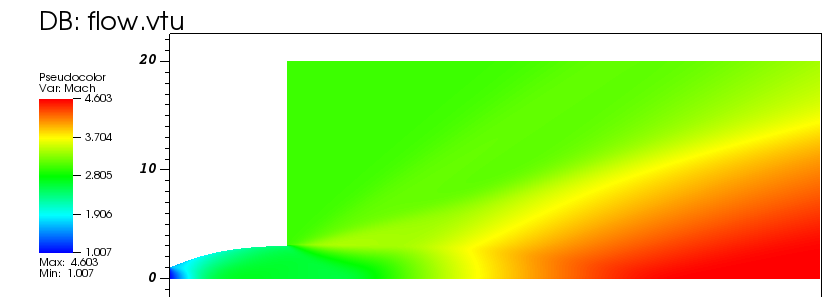
\includegraphics[width=0.75\textwidth]{text/Mach contour 1.png}
    \caption[Mach Contour of Extended Mesh II]{Mach Contour}
    \label{fig:Mach Contour}
\end{figure}
Though the exit parameters match the required optimum conditions, due to the incorrect initial conditions at the domain outside the nozzle the flow develops expansion fans.\\
\\
\\
(C) Optimum Expanded Nozzle: The \textbf{pressure outlet} boundary condition is replaced as \textbf{farfield}. The freestream values are P$_{e6}$ and atmospheric temperature \textcolor{red}{3000 K}\\
\begin{figure}[H]
    \centering
    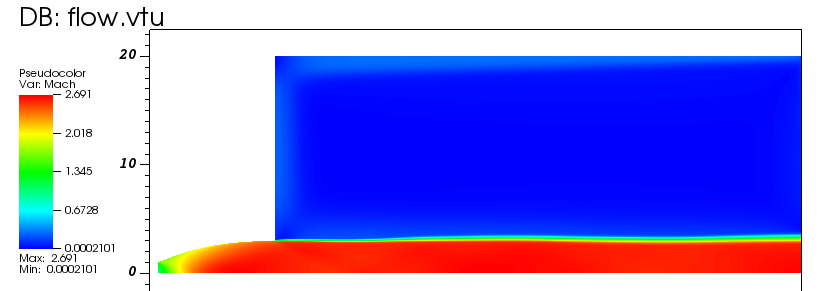
\includegraphics[width=0.75\textwidth]{text/Mach_ROE_Success.png}
    \caption[Mach Contour of Extended Mesh III]{Mach Contour}
    \label{fig:Mach Contour}
\end{figure}
\begin{table}[ht]
    \centering
    \begin{tabular}{|c|c|}
    \hline
    T_{o}  &  3600 \\
    \hline
    P_{o} & 7 Mpa\\
    \hline
    P$_{e}$/P$_{th}$ & 0.0473  \\
    \hline
    \end{tabular}
    \caption{Parameters}
    \label{tab:my_label}
\end{table}
\\
(D) Under-Expanded Nozzle: he \textbf{pressure outlet} boundary condition is \textbf{farfield}. The freestream values are P$_{exit}$ = 1 atm and atmospheric temperature \textcolor{red}{3000 K}
\begin{figure}[H]
    \centering
    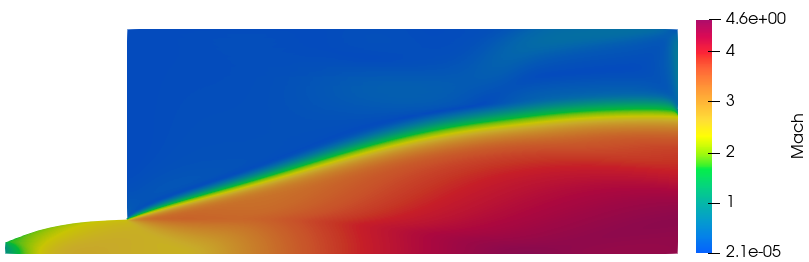
\includegraphics[width=0.75\textwidth]{text/Mach_Underexpanded Nozzle.png}
    \caption{Mach Contour Under-Expanded Nozzle}
    \label{Mach Contour Under-Expanded Nozzle}
\end{figure}
The initial condition on temperature seems to be the crucial parameter as it produces converging residuals. Altering this value to any other value either gives unsteadiness in the flow or produces viscous like effect. \\

(E) Under-Expanded Nozzle: he \textbf{pressure outlet} boundary condition is \textbf{farfield}. The freestream values are P$_{exit}$ = 500000 Pa and atmospheric temperature \textcolor{red}{3000 K}
\begin{figure}[H]
    \centering
    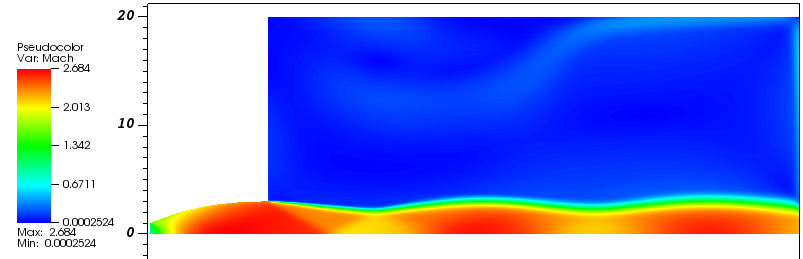
\includegraphics[width=0.75\textwidth]{text/Mach_Overexpanded Nozzle.png}
    \caption{Mach Contour Over-Expanded Nozzle}
    \label{Mach Contour Over-Expanded Nozzle}
\end{figure}

\newpage
\begin{flushleft}
\textbf{Results and Analysis}\\
\end{flushleft}
The initial condition for temperature is strictly incorrect for the entire domain that is present outside the nozzle as the temperature outside the nozzle is just 288 kelvin and pressure is P$_{e6}$. But the prime reason to take this approach is to ensure that the inlet initial condition meets the required mach number, i.e., 1. There is no clear picture to understand how SU2 calculates the inlet mach number with the given boundary conditions and initial condition. One hypothesis is that with the given total conditions SU2 might assume isentropic flow and it evaluates the mach number as 2.64 at the outlet. This value may be used to back calculate the mach number at the inlet. But when the free-stream temperature is assigned 288 K, the residual starts to \textbf{oscillate}. One hypothesis could be the Mach number which is calculated from P$_{e6}$ and T$_0$ must be same for physical consistency.\\
\newpage

\section{Method Of Characteristics}
\label{section:trabrelacionados}
\subsection{Theory of MoC}
The key assumptions are the flow is inviscid and irrotational. For such flows the complete velocity governing equation can be written as:\\
\begin{center}
    $ (1 - \frac{u^2}{a^2})\frac{\partial u}{\partial x} + (1 - \frac{v^2}{a^2})\frac{\partial v } {\partial y } - \frac{2uv}{a^2}\frac{\partial du}{\partial dy} = 0$
\end{center}\\
The velocity of any supersonic flow can be broken down such that one of its two components has speed of sound, from the above equation when $u$ equals $a$, $\frac{\partial u}{\partial x}$ becomes indeterminate, and it remains indeterminate along the line $\sin{\mu} = \frac{a}{V}$. Such lines are called characteristic lines, which are also the mach waves. It can be shown that
\begin{center}
    $ (\frac{dy}{dx})_{char} = \tan(\theta \mp \mu) $\\
    $  \theta + \nu(M) = K$_-$  $\\
    $  \theta - \nu(M) = K$_+$  $\\
\end{center}
\begin{figure}[H]
    \centering
    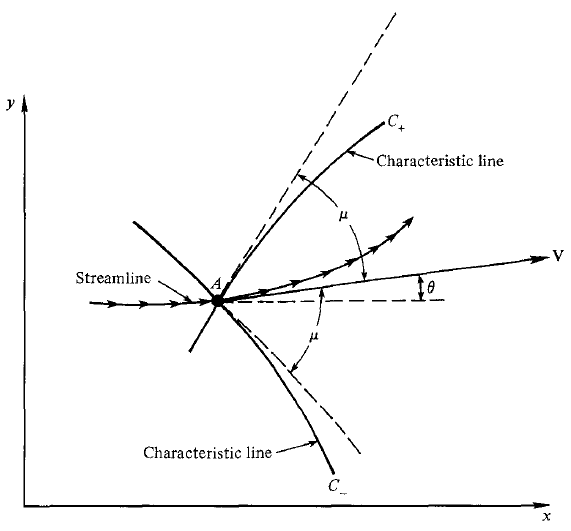
\includegraphics[width=0.5\textwidth]{text/Characteristic lines.PNG}
    \caption[Characteristic line]{Slope of characteristic line (Source [1])}
    \label{fig:Slope of characteristic line}
\end{figure}
When two characteristics are intersecting at a point, then the flow angle $\theta$ and prandlt meyer function $\nu$ can be estimated using\\
\begin{center}
    $  \theta_1 + \nu(M)_1 = K$_-$_1 = K$_-$_3 = \theta_3 + \nu(M)_3 $\\ 
    $  \theta_2 - \nu(M)_2 = K$+-$_1 = K$+-$_3 = \theta_3 - \nu(M)_3 $\\ 
    \end{center}
\begin{figure}[H]
    \centering
    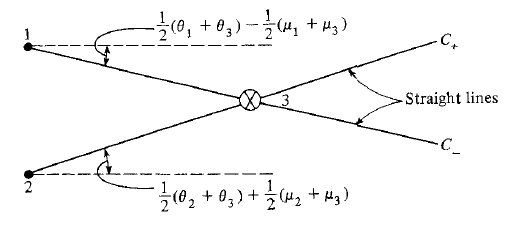
\includegraphics[width=0.5\textwidth]{text/intersection_characterisitcs.PNG}
    \caption[Intersection of Characteristics]{Intersection of Characteristics (Source [1])}
    \label{fig:Intersection of Characteristics}
\end{figure}    
Assuming the slope angle of mach lines is the average of the slope angles, the coordinates of the third point can be calculated from\\
\begin{center}
    $\frac{y_3 - y_2}{x_3 - x_2} = \tan(0.5(\theta_3 + \theta_2) + 0.5(\nu_3 + \nu_2) )  $\\
    $\frac{y_3 - y_1}{x_3 - x_1} = \tan(0.5(\theta_3 + \theta_1) - 0.5(\nu_3 + \nu_1) )  $\\
\end{center}
\subsection{Nozzle Design}
Key assumptions
\begin{enumerate}
\setlength\itemsep{0.01em}
    \vspace{-2mm}
    \item Inviscid and Irrotational
    \vspace{-2mm}
    \item Characteristics are only slightly curved
\end{enumerate}
The diverging section of the nozzle generally consists of expansion section and straightening section. The slope of the nozzle contour at the expansion fan is continuously increasing, or in other words the function of the nozzle contour at the expansion section is monotonously increasing hence it generates expansion waves and as well as reflects the incident expansion waves. The slope of the nozzle contour at the straightening section is monotonously decreasing, hence it terminates all the expansion waves incident on it. So the junction of expansion and straightening section has the highest slope($\theta_{max}$) in the nozzle wall contour. For a minimum length nozzle there is only a straightening section, as expansion section would just add on to excess mass. Henceforth the word nozzle is used instead of minimum length nozzle. At the throat there is a discontinuity in the slope of the nozzle contour. At this junction expansion fan emanates, which consists of series of expansion waves. At point 'A'\\
\\
   \theta$_{exp}$ = \nu(M$_2$) - \nu(M$_1$)\\
    \theta$_{max}$ = \nu$_A$ | Since 'A' is a sonic point, $\nu(M = 1) = 0$, hence K$_+$ = 0\\
    \theta$_{max}$ + \nu$_A$ = (K$_-)_A$\\ 
    (K$_-)_A$ = \theta$_{exit}$ + \nu$_{exit}$ as both the points lie on the same characteristic\\
    \theta$_{exit}$ = 0 | Imposing the condition that the flow has to emerge parallel to the center at the exit
    line\\
    \theta$_{max}$ = \nu$_A$ = \nu$_{exit}$/2\\
\\
\begin{figure}[H]
    \centering
    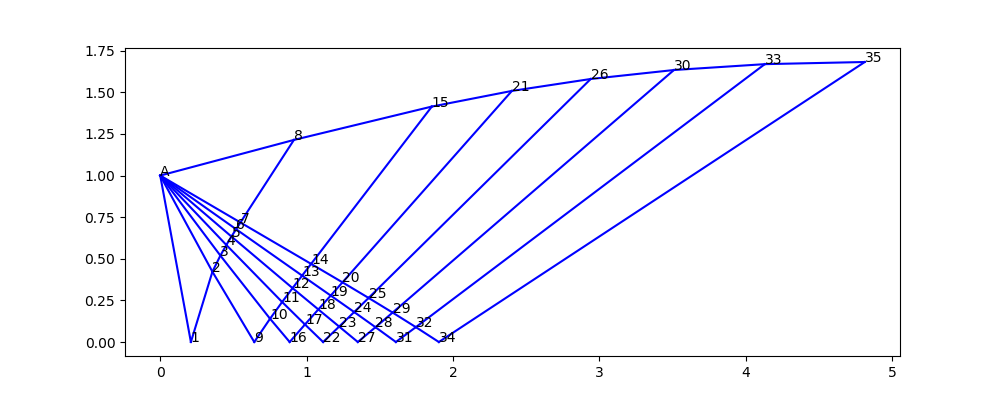
\includegraphics[width=1\textwidth]{text/MoC_Mine_Blue.png}
    \caption{Minimum Length Nozzle}
    \label{fig:Minimum Length Nozzle}
\end{figure}
So to design a nozzle, the first requirement is the exit mach number. And the slope at the throat corner point is decided by the prandlt meyer function at the exit point. All the points on the centerline has $\theta$ as zero, hence the mach number at the last point lying on the centerline has the same mach number as the design exit mach number. For the supersonic nozzle design, the algorithm to find the nozzle contour is as follows:
\begin{enumerate}
\setlength\itemsep{0.01em}
    \item Design the exit mach number and evaluate $\theta_{max}$
    \item Decide the number of characteristics required, say N
    \item At point 1, we assume$\dag$ $\theta_1$ a finite non-zero value, say 0.01$^0$, since K_+ = 0, \theta$_1$ = \nu$_1$ for all the points 1, 2... N, N+1
    \item We assume$\dag$  that for points 2,3...N flow angle $\theta$ is $\Delta\theta$ = $\theta_{max}/(N-1)$ inclined with $\theta_1$
    \item Assume the first set of characteristics are straight lines
    \item There are two approaches to find the slope:
    \begin{enumerate}
        \item Assuming the angle between the characteristics is also $\Delta\theta$
        \begin{enumerate}
            \item $\frac{x_i - x_a}{y_a - y_i} = \tan(\theta_i+\theta_1)$ for all i $\in {2...N}$    
        \end{enumerate}
        \item Assuming the slope angle of the line has contribution only from the points 1,2...N
        \begin{enumerate}
            \item $\frac{y_i - y_a}{x_i - x_a} = \tan(\theta_i - \nu_i )$ for all i $\in {1,2...N} $
        \end{enumerate}
    \end{enumerate}
    \item For contour points $0.5(\theta_a + \theta_i)$ is the slope angle
\end{enumerate}\\

\begin{figure}[H]
    \centering
    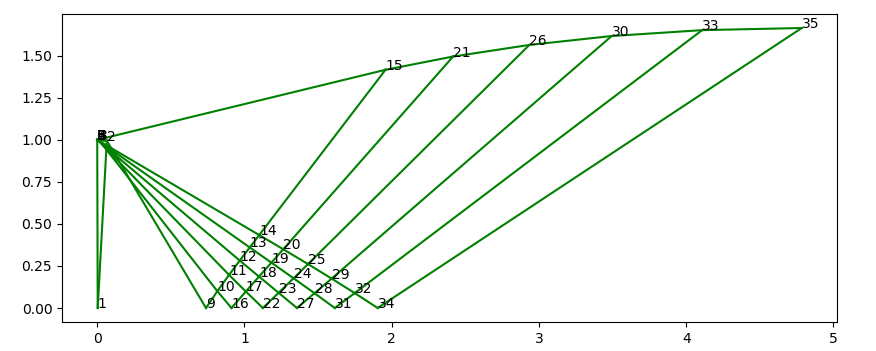
\includegraphics[width=0.8\textwidth]{text/MoC_Anderson.PNG}
    \caption[MOC Method I]{MOC Method I}
    \label{fig:MOC Method I}
\end{figure}

\begin{figure}[H]
    \centering
    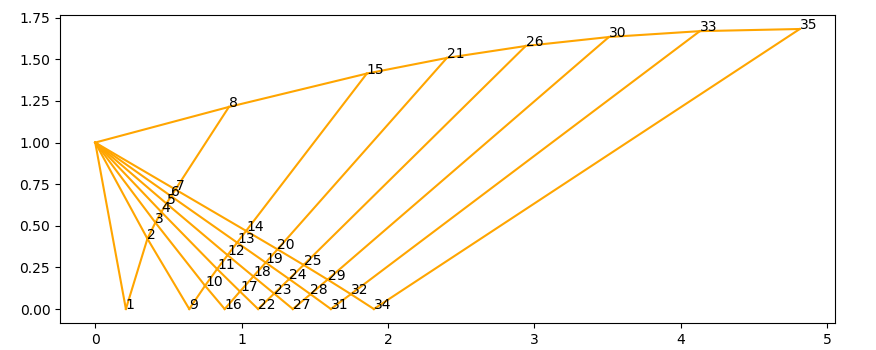
\includegraphics[width=0.8\textwidth]{text/MoC_Mine.png}
    \caption[MOC Method II]{MOC Method II}
    \label{fig:MOC Method I}
\end{figure}\\
\newpage
\begin{flushleft}
\textbf{Convergence}\\
\end{flushleft}
The values of Area ratio and length of the Nozzle converges when Number of Characteristics is about 30. But the variation is small even at lower number of characteristics. \\
\begin{center}
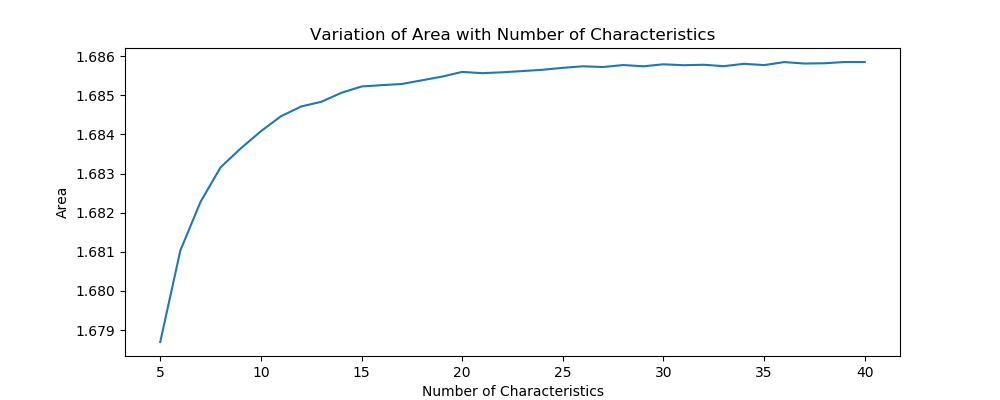
\includegraphics[width=0.8\textwidth]{text/Area Variation.png}\\
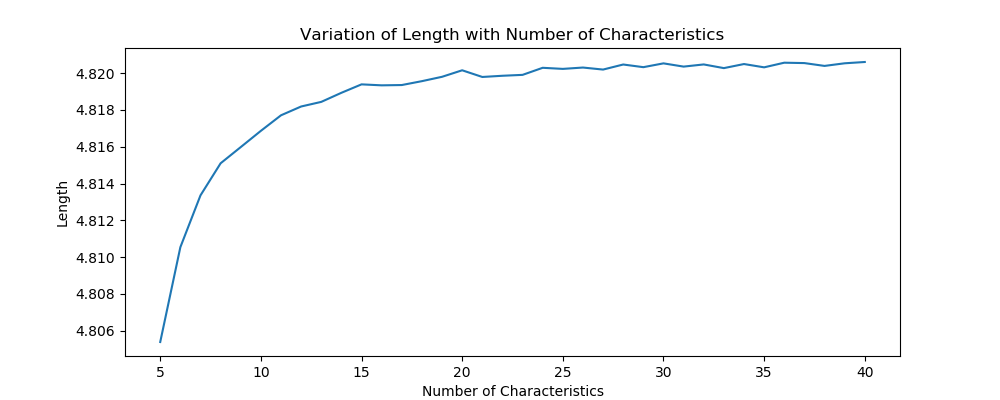
\includegraphics[width=0.8\textwidth]{text/Length Variation.png}\\    
\end{center}


\newpage
%\subsection{Nozzel Simulation using Time-Marching MacCormack Techinque}

\begin{flushleft}
{\bf \huge Future Work} \\[1em] 
\end{flushleft}
The mathematics aspect of the numerical schemes are yet to be explored. In the subsequent week the simulation of the 2-D nozzle using Time Marching MacCormack's technique will be performed. \\
\\
\textbf{MacCormack Technique}\\
%\vspace{-2 mm}
Let's say the Initial Conditions are known on a vertical line, and there are no source terms
\begin{itemize}
\setlength\itemsep{0.01em}
    \item $\frac{\partial F}{\partial x} = -\frac{\partial G}{\partial y} $
    \item $ F_{i+1} = F_{i} + \frac{\partial F}{\partial x}_{avg}\Delta x  $
    \item $\frac{\partial F}{\partial x}_{avg} = 0.5*(\frac{\partial F}{\partial x}_{i,j}+\frac{\partial F}{\partial x}_{i+1,j}) $
\end{itemize}
\\
\begin{itemize}
\setlength\itemsep{0.01em}
    \item First $ F_{i+1}$ is evaluated using $ \overline{F_{i+1}} = F_{i} + \frac{\partial F}{\partial x}_{i,j}\Delta x  $
    \item Predictor Step: $\frac{\partial F}{\partial x}_{i,j}$ is obtained from $\frac{\partial G}{\partial y}_{i,j} $ using a forward difference $\hat{j}$
    \item $\overline{F}_{i+1}$ is used to evaluate $\overline{G}_{i+1}$
    \item Corrector Step: $\frac{\partial F}{\partial x}_{i+1,j}$ is obtained from  $\frac{\partial \overline{G}}{\partial y}_{i+1,j} $ using a rearward difference along $\hat{j}$
    \item Even though each of the predictor and corrector step are first order, the overall scheme is second order as in the $\frac{\partial F}{\partial x}_{avg}$ the $\Delta x$ terms cancel due to averaging
\end{itemize}
The same technique can be applied with a small modification by adding the unsteady term, and initial condition is known at the sonic line at the throat of the nozzle. The rest of the initial conditions are assumed arbitrarily in some fashion. \\
\begin{figure}[H]
    \centering
    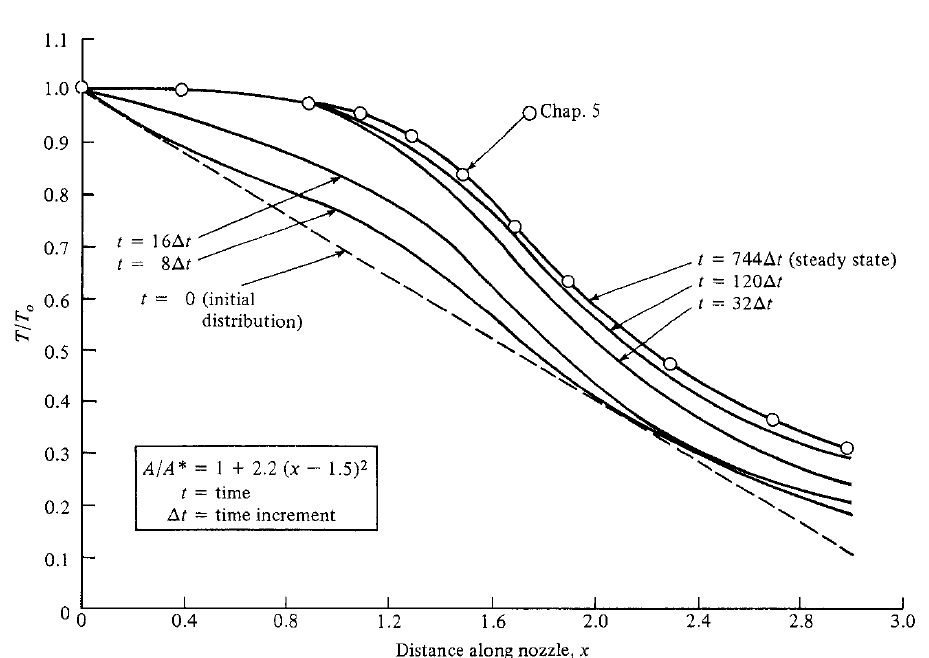
\includegraphics[width=0.75\textwidth]{text/time marching.PNG}
    \caption{Time Marching}
    \label{fig:Time Marching}
\end{figure}


\newpage


\bibliographystyle{apalike}
\bibliography{bibliography.bib}
$[1]$ Modern Compressible Flows by John D. Anderson, Jr\\
$[2]$ SU2 Official Documentation \url{https://su2code.github.io/docs_v7/}\\
$[3]$ CFD Discussion Forum \url{https://www.cfd-online.com/Forums/su2/}\\
$[4]$ CFD Blog \url{http://www.joshtheengineer.com/2018/02/28/how-to-run-su2-start-to-finish/}
\end{document}